\chapter{Thermal Expansion}
\label{ch:thermalExpansion}

\section{Necessity of Modeling}
  % discuss the EBR-II tests
  % todo find sources for EBR-II & PRISM
  The Sodium Cooled Fast Reactor (SFR) as modeled is entirely composed of
  metals and, as such, experience significant thermal expansion. While other 
  designs may employ different fuel material, these are not considered. Such
  reactor designs composed of metal fuel include Experimental Breeder Reactor II
  (EBR-II) as designed and built by Argonne National Laboratory (ANL) as well as
  GE-Hitachi Nuclear Energy's PRISM. 

  \cite{PlentifulEnergy}

\section{Model Details}
  Highly detailed thermal expansion modeling can be done using the Finite
  Element Method to calculate local stresses and strains on all reactor
  structural components. However, the model developed here for the simulation of
  SFRs does not estimate temperature and heat generation at all positions due to
  the smearing of hexagonal assemblies. Therefore, a simplified thermal
  expansion model is developed to simulate the effect of thermal expansion on
  reactivity.

  In the model, linear dimensions are expanded based on material properties.
  All sodium in the reactor is assumed to be liquid so effects of thermal
  expansion within the sodium are assumed to be described by the change in
  density as a function of temperature as described by state equations in
  \cite{sodiumProp}. Additionally, the mass of sodium within the reactor is not
  conserved. Sodium in the coolant is allowed to flow into and out of an
  expansion vessel external to the reactor. In a SFR, sodium in the bond region
  flows upward from the fuel region into a gas plenum; however, this is not
  modeled as the sodium level in the bond is not tracked. Instead, the mass of
  sodium in the bond region is allowed to vary during the simulation.

  All structural materials in the reactor are modeled as HT9 stainless steel.
  Fuel material is modeled as metallic uranium with 10\% Zr by weight included
  (i.e. U10Zr). Thermal expansion properties for HT9 are given in \cite{ht9Prop}
  and for U10Zr are given in \cite{thexpU10Zr}. The equations for the Linear
  Expansion Factor (LEF) as functions of temperature as used in this application 
  are given
  \begin{equation}
    \label{eq:lef_ht9}
    \left( \frac{\Delta L}{L} \right)_{\text{HT9}} = 
      -2.191 \times 10^{-3} + 5.678 \times 10^{-6} \, T + 
      8.111 \times 10^{-9} \, T^2 - 2.576 \times 10^{-12} \, T^3 
  \end{equation}
  \begin{multline}
    \label{eq:lef_u10zr}
    \left( \frac{\Delta L}{L} \right)_{\text{U10Zr}} = \\
      \begin{cases}
        -7.3 \times 10^{-3} + 3.489 \times 10^{-5} \, T 
          - 5.154 \times 10^{-8} \, T^2 + 4.39 \times 10^{-11} \, T^3 & 
          T \le 923 \units{K} \\
        -0.25252 + 6.669 \times 10^{-4} \, T - 5.441 \times 10^{-7} \, T^2 
          + 1.518 \times 10^{-10} \, T^3 & \text{otherwise}
      \end{cases}
  \end{multline}
  for $T$ in \units{K}. Note that U10Zr has a phase change at 923 \units{K} that 
  increases the LEF at this point. The LEF of HT9 and U10Zr over the range of
  operating temperatures of SFRs are plotted in \fref{fig:lef_plot}.  It is 
  observed that the LEF of U10Zr is as much as twice that of HT9. This implies
  fuel material will expand significantly more than structural material which is
  expected behavior for metallic fuel.

  \begin{figure}
    \centering
    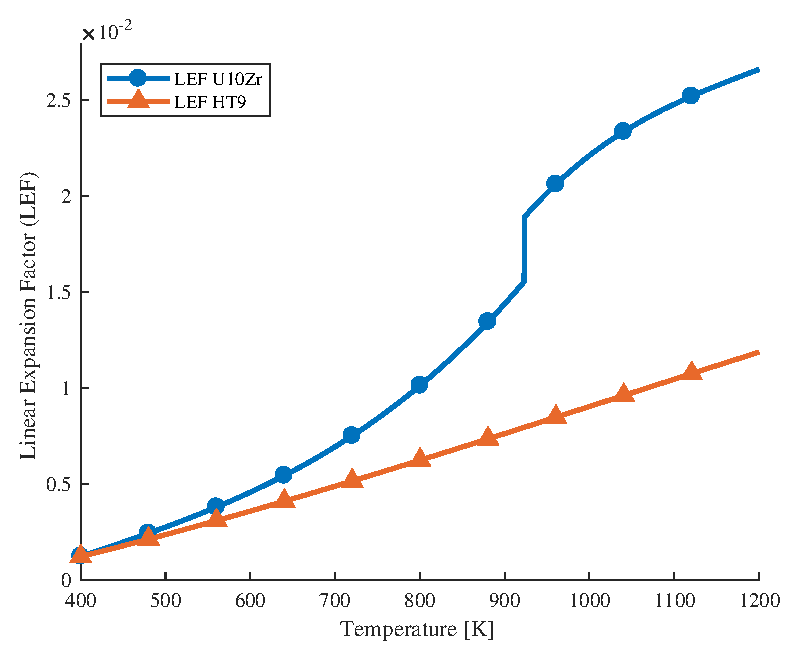
\includegraphics[width=0.7\textwidth]{lef_plot}
    \caption{Linear Expansion Factor for HT9 Steel and U10Zr Fuel.}
    \label{fig:lef_plot}
  \end{figure}

  To simplify the modeling of thermal expansion, material dimensions are
  uniformly expanded in radial and axial directions. It is assumed that material
  expansion in the radial direction (both $x$ and $y$ directions) expands
  as HT9 because the dominating expansion in this direction is
  due to the expansion of the hexagonal assemblies themselves. It is assumed 
  that material expansion in the axial direction (the $z$ direction) expands
  as U10Zr because the dominating expansion in this direction is the elongation
  of the metallic fuel. Within a hexagonal assembly, all dimensions are expanded
  as HT9 with the exception of the fuel radius, $R_F$, which is expanded as 
  U10Zr. Within a hexagonal assembly, the coolant flow area and the sodium bond
  area are allowed to ``float'' because they are assumed liquid. All dimensions
  in the reactor are expanded assuming the user-input dimensions are at
  room-temperature conditions and using a single, fixed thermal expansion
  temperature $T_{exp}$. The expansion temperature should be selected to
  represent the average temperature within the reactor. It is expected thermal
  expansion effects will be significant. However, thermal expansion factors are
  typically on the order $10^{-6}$ so small, local changes in temperature are
  not expected to affect the macroscopic simulation.

  Given the assumptions of this model, a radial thermal expansion factor can be
  defined using \eref{eq:lef_ht9} as
  \begin{equation}
    \label{eq:lef_r}
    F_r(T_{exp}) = \left(\frac{\Delta L}{L}\right)_{\text{HT9}}
  \end{equation}
  which is a function of $T_{exp}$. Note that given the assumption of uniform
  radial thermal expansion, ${F_x(T_{exp}) = F_y(T_{exp}) = F_r(T_{exp})}$.
  Similarly, an axial thermal expansion factor can be defined using
  \eref{eq:lef_u10zr} as 
  \begin{equation}
    \label{eq:lef_a}
    F_a(T_{exp}) = \left(\frac{\Delta L}{L}\right)_{\text{U10Zr}}
  \end{equation}
  and $F_a(T_{exp}) = F_z(T_{exp})$. For a ``cold'' cooridnate $(x^C,y^C,z^C)$,
  the thermally expanded ``hot'' coordinate $(x^H,y^H,z^H)$ can be expressed 
  using radial and axial thermal expansion factors as
  \begin{align}
    \label{eq:expand_x}
    x^H &= x^C + x^C \, F_r(T_{exp}) \\
    \label{eq:expand_y}
    y^H &= y^C + y^C \, F_r(T_{exp}) \\
    \label{eq:expand_z}
    z^H &= z^C + z^C \, F_a(T_{exp})
  \end{align}
  which is consistent with the assumption of uniform radial and axial expansion.

  Using the coordinate transforms in \eref{eq:expand_x}, \eref{eq:expand_y}, and
  \eref{eq:expand_z}, consider the thermal expansion of a cold volume $V^C$.
  Volume $V^C$ has coordinate components $L_x^C$, $L_y^C$, and $L_z^C$ such that 
  ${V^C = L_x^C \, L_y^C \, L_z^C}$. Then, the thermally expanded volume $V^H$ 
  can be written
  \begin{align}
    V^H &= V^C + \Delta V, \\
    V^H &= (L_x^C + \Delta L_x) (L_y^C + \Delta L_y) (L_z^C + \Delta L_z). 
  \end{align}
  Then, recognizing the coordinate expansions 
  ${\Delta L_x = L_x^C F_r(T_{exp})}$.
  \begin{align}
    V^H &= (L_x^C + L_x^C \, F_r(T_{exp})) + (L_y^C + L_y^C \, F_r(T_{exp})) + 
      (L_z^C + L_z^C \, F_a(T_{exp})) \\
    V^H &= L_x^C \, L_y^C \, L_z^C \, (1 + F_r(T_{exp}))^2 (1+F_a(T_{exp})) \\
    V^H &= V^C (1 + F_r(T_{exp}))^2 (1+F_a(T_{exp}))
  \end{align}
  The volume ratio is then
  \begin{equation}
    \label{eq:volume_ratio}
    \frac{V^C}{V^H} = \frac{1}{(1+F_r(T_{exp}))^2 (1+F_a(T_{exp}))}.
  \end{equation}
  Given the assumption of uniform thermal expansion in axial and radial
  directions, the ratio of volumetric expansion is constant throughout the
  reactor.

  It is assumed that the cross-sectional area of the hexagonal assembly is 
  confined to the radial direction; any warping of the assembly that would
  violate this assumption is neglected. Then, the hexagonal assembly has total
  cross-sectional area $A$ and contains component cross sections $A_i$. For
  example, the total area occupied by the fuel material could be considered
  $A_i$ and the total area of the hexagon described by the flat-to-flat
  dimension could be considered $A$. Define $A_i$ such that $\sum_{i} A_i = A$.
  Let the fractional area $a_i = A_i/A$ and $\sum_{i} a_i = 1$.

  Similar to a ratio of volumetric expansion, a ratio of area expansion may be
  derived. Assume all dimensions in the radial direction (to which the
  cross-sectional assembly area is confined), expand according to
  $F_r(T_{exp})$. Then, consider a representative area $A^C = L_x^C L_y^C$.
  Then, the thermally expanded volume $A^H$ can be written
  \begin{align}
    A^H &= A^C + \Delta A, \\
    A^H &= (L_x^C + \Delta L_x) (L_y^C + \Delta L_y).
  \end{align}
  Recognizing the coordinate thermal expansions ${\Delta L_x = L_x^C
  F_r(T_{exp})}$.
  \begin{align}
    A^H &= (L_x^C + L_x^C F_r(T_{exp})) (L_y^C + F_r(T_{exp})) \\
    A^H &= L_x^C L_y^C (1 + F_r(T_{exp}))^2 \\
    A^H &= A^C (1 + F_r(T_{exp}))
  \end{align}
  The area ratio is then
  \begin{equation}
    \label{eq:area_ratio}
    \frac{A^H}{A^C} = (1 + F_r(T_{exp}))^2.
  \end{equation}

  Consider the thermal expansion of area fractions $a_i$. Observe $a_i^C =
  \frac{A_i^C}{A^C}$. Then, both $A_i$ and $A$ are thermally expanded according
  to \eref{eq:area_ratio}.
  \begin{align}
    a_i^H &= \frac{A_i^H}{A^H} \\
    a_i^H &= \frac{A_i^C (1 + F_r(T_{exp}))^2}{A^C (1 + F_r(T_{exp}))^2} \\
    \label{eq:constant_area_frac}
    a_i^H &= a_i^C
  \end{align}
  \eref{eq:constant_area_frac} implies that for uniform thermal expansion in the
  radial directions, area fractions are unaffected by thermal expansion though
  areas themselves expand. 
  
  However, in the model used here, the fuel radius and fuel area
  are expanded according to $\left(\frac{\Delta L}{L_0}\right)_{\text{U10Zr}}$
  whereas all other materials are expanded according to 
  $\left(\frac{\Delta L}{L_0}\right)_{\text{HT9}}$. This does imply that,
  numerically, the radius of the fuel could exceed the inner radius of the clad
  which is a non-physical result. This will only happen for small sodium bond
  gaps and high thermal expansion temperatures. In these cases, the radius of
  the fuel is confined to the expanded inner radius of the cladding. Though a
  more complex relationship describes the true value of these radii, the error
  due to this assumption is small compared to the assumption of uniform thermal
  expansion.
  
  Due to the different thermal expansions of fuel and structural material within
  the cross-section of the hexagonal assembly, the thermal expansion of area 
  fractions does not obey \eref{eq:constant_area_frac}. Instead, area fractions
  are simply calculated at hot and cold conditions and the ratio from this
  calculation is used.

\section{Implementation}
  Thermal expansion effects the reactor simulation in two major ways. First,
  thermal expansion causes the physical dimensions of the reactor to increase. 
  This is modeled by the expansion of individual elements in the solution of the
  neutron diffusion equation via the finite element method (see
  \chref{ch:neutronDiffusion}) as well as the expansion of areas within the 
  hexagons.  Second, as a result in the increase in physical dimensions, the 
  density of reactor materials decreases. This decrease in density is necessary
  to preserve the quantity of material within the reactor. In this derivation,
  the number of atoms are conserved. The density change due to thermal expansion 
  is observed as an effect on cross-sections.

  \subsection{Expansion of Elements and Area Fractions}
    Given the assumption of constant thermal expansion in radial and axial
    directions, thermal expansion is straightforward. Each node coordinate in
    the mesh is expanded according to \eref{eq:expand_x}, \eref{eq:expand_y},
    and \eref{eq:expand_z}. By expanding in axial and radial directions
    uniformly throughout the reactor, it is certain that there will be no
    intersection or overlap of elements. In a realistic analysis, stress,
    strain, and contact pressures must be accounted for but this is unnecessary
    here because the assumptions prohibit overlap and intersection conditions.

  \subsection{Cross-section Effects}
    The conservation of reactor material is expressed as a conservation of 
    number of atoms. Allow the superscript $H$ to represent ``hot'' conditions 
    (i.e.  thermally expanded) and the superscript $C$ to represent ``cold'' 
    conditions.  Then, the conservation of the number of atoms for species $i$, 
    can be expressed as
    \begin{equation}
      \label{eq:conservation}
      n_i^H = n_i^C 
    \end{equation}
    where $n_i^H$ is the number of atoms of species $i$ after thermal expansion.
    The number of atoms $n_i$ can be written as 
    \begin{equation}
      \label{eq:nden_definition}
      n_i = N_i \, V_i
    \end{equation}
    where $N_i$ is the number density of species $i$ and $V_i$ is the volume
    occupied by species $i$. Then, inserting \eref{eq:nden_definition} into 
    \eref{eq:conservation} yields an expression for the thermally expanded 
    number density of species $i$ as
    \begin{align}
      N_i^H \, V_i^H &= N_i^C \, V_i^C, \\
      N_i^H &= N_i^C \frac{V_i^C}{V_i^H}
    \end{align}
    where the term $\frac{V_i^C}{V_i^H} < 1$ and represents the expansion of the
    volume occupied by species $i$. Using the relationship from
    \eref{eq:volume_ratio}
    % todo


\section{Results}
  \begin{figure}
    \centering
    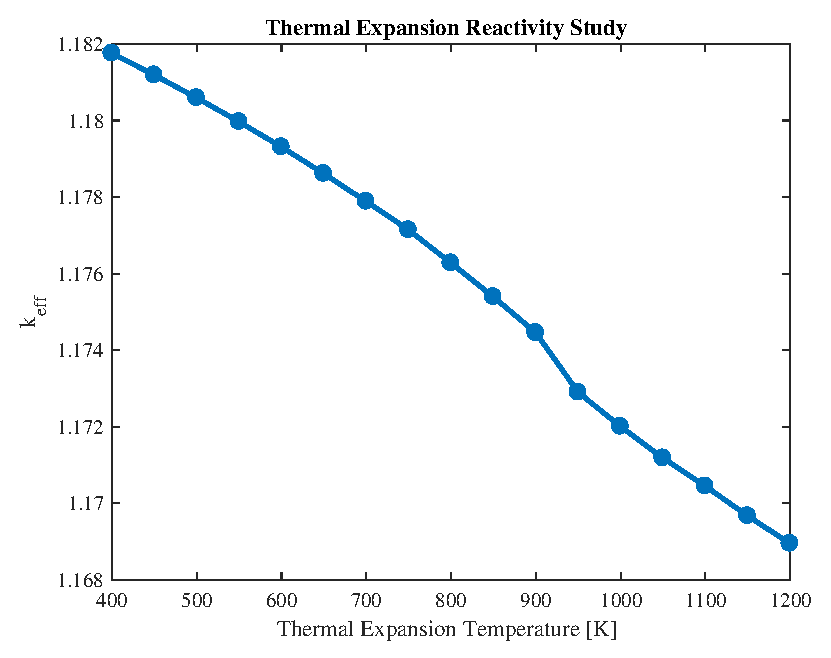
\includegraphics[width=0.7\textwidth]{thexp_study}
    \caption{Reactivity due to Thermal Expansion Temperature.}
    \label{fig:thexp_study}
  \end{figure}

